\section{Stochastic Loads Method (Long Run)}
This solution was run with a targeted execution time of approximately 2.5 hours. The solution was calculated using the following command line arguments to the solver: 

\begin{verbatim}
python -m pystruct <<data_file>>  -S3 -i80 -g200 --csv
\end{verbatim}

\noindent Where: 

\begin{itemize}
  \item \codeword{-S3}: Select solution 3: Stochastic Loads Method
  \item \codeword{-i80}: Use a population size of 80. 
  \item \codeword{-g200}: Use a generation count of 200. 
  \item \codeword{--csv}: Generate CSV output for final Pareto Front
\end{itemize}


\subsection{Resultant Pareto Front}
Table \ref{tab:pfront_sto} shows the design parameters of the members of the Pareto Front generated by this solution run. The Pareto Front is also given graphically in Figure \ref{fig:pfront_sto}. 
\begin{table}[!htbp]
\centering
\small
\begin{tabular}{|p{1.5cm}p{1.5cm}p{1.4cm}p{2cm}p{2cm}p{1.5cm}p{1.5cm}|}
\hline
Top Flange Width&Bottom Flange Width&Web Thickness&Doubler Thickness at Hoist Pin&Doubler Thickness at Load Pin&Reliability Index& Mass\\
\hline
mm&mm&mm&mm&mm&ul&kg\\
\hline
91.997&101.419&6.724&43.826&243.824&3.095&265.219\\
91.526&236.107&78.99&33.03&89.924&6.481&783.150\\
80.127&253.897&20.274&19.704&78.611&5.672&333.867\\
49.012&277.521&86.506&43.241&216.625&6.688&900.125\\
174.133&194.853&30.888&18.281&107.054&5.815&437.764\\
35.949&103.641&76.501&32.843&249.291&6.298&756.122\\
51.253&118.064&7.176&87.576&30.322&3.065&203.018\\
63.211&102.335&18.535&14.396&127.905&4.316&269.780\\
132.862&263.599&60.726&106.691&219.739&6.516&787.654\\
169.514&201.544&73.331&34.801&246.143&6.554&825.922\\
207.564&215.857&71.357&30.79&87.27&6.439&762.066\\
89.162&261.263&91.525&48.149&244.42&6.73&962.654\\
55.855&58.564&2.359&90.19&8.066&-0.7825&137.751\\
87.785&198.101&44.651&44.423&133.73&6.042&538.436\\
78.561&223.986&52.554&30.01&171.362&6.268&608.499\\
72.355&246.809&29.056&20.85&59.901&5.787&386.186\\
\hline
\end{tabular}
	\caption{Members of the Pareto Front generated through Stochastic Loads (Long Run)}
\label{tab:pfront_sto}
\end{table}

\begin{figure}
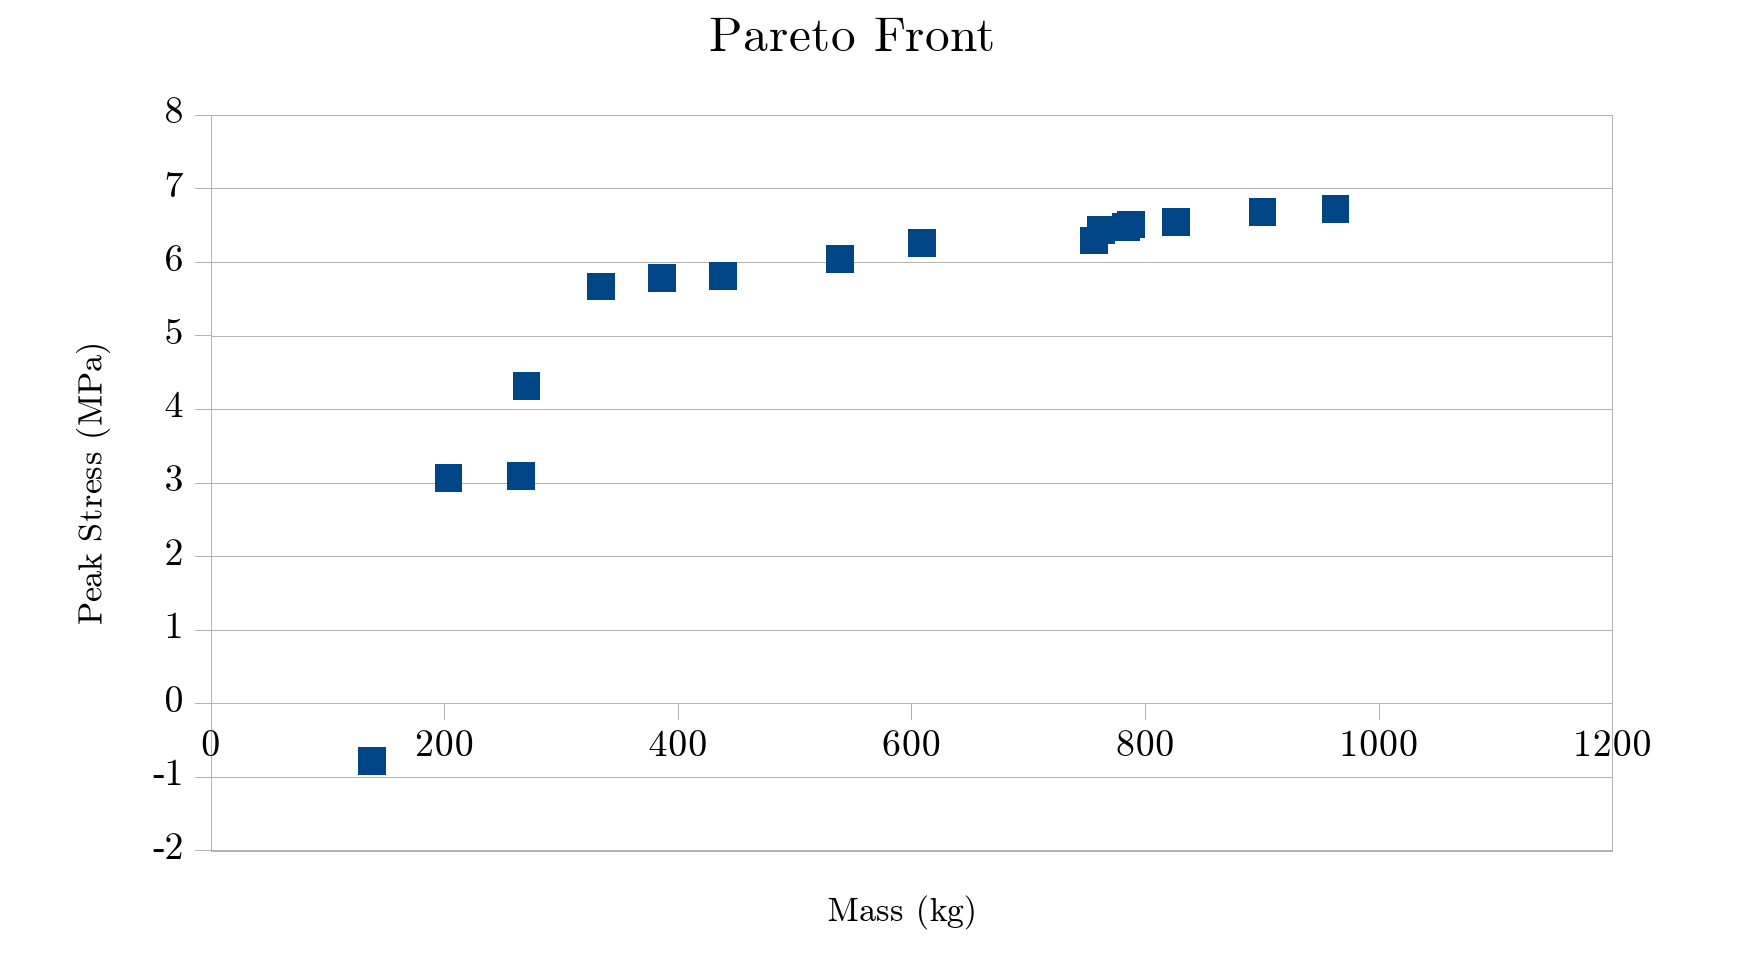
\includegraphics[width=\textwidth]{img/s3i80g200_front.png}
	\caption{Graph of the Pareto Front generated through Stochastic Loads (Long Run)}
\label{fig:pfront_sto}
\end{figure}

\subsection{Solution Statistics}
This solution also was tracked for several computing performance indicators to compare the performance of the algorithm with the other solutions. These statistics are listed in Table \ref{tab:stat_sto}. 

\begin{table}[!htbp]
  \centering
  \begin{tabular}{|l|l|}
    \hline
	  Total Generations Computed & 200\\
    Average Time Per Generation (sec) & 44.6\\
    Total Wall Clock Time (sec)	 & 8.92E+03\\
    \hline
  \end{tabular}
	\caption{Solution Statistics for Stochastic Loads (Long Run)}
  \label{tab:stat_sto}
\end{table}


\section{Stochastic Loads Method (Short Run)}
This solution was run with a targeted execution time of approximately 1.5 hours. The solution was calculated using the following command line arguments to the solver: 

\begin{verbatim}
python -m pystruct <<data_file>>  -S3 -i80 -g110 --csv
\end{verbatim}

\noindent Where: 

\begin{itemize}
  \item \codeword{-S3}: Select solution 3: Stochastic Loads Method
  \item \codeword{-i80}: Use a population size of 80. 
  \item \codeword{-g110}: Use a generation count of 110. 
  \item \codeword{--csv}: Generate CSV output for final Pareto Front
\end{itemize}


\subsection{Resultant Pareto Front}
Table \ref{tab:pfront_sto_short} shows the design parameters of the members of the Pareto Front generated by this solution run. The Pareto Front is also given graphically in Figure \ref{fig:pfront_sto_short}. 

\begin{table}[!htbp]
\centering
\small
\begin{tabular}{|p{1.5cm}p{1.5cm}p{1.4cm}p{2cm}p{2cm}p{1.5cm}p{1.5cm}|}
\hline
Top Flange Width&Bottom Flange Width&Web Thickness&Doubler Thickness at Hoist Pin&Doubler Thickness at Load Pin&Reliability Index& Mass\\
\hline
mm&mm&mm&mm&mm&ul&kg\\
\hline
\hline
\end{tabular}
	\caption{Members of the Pareto Front generated through Stochastic Loads (Short Run)}
\label{tab:pfront_sto_short}
\end{table}

\begin{figure}
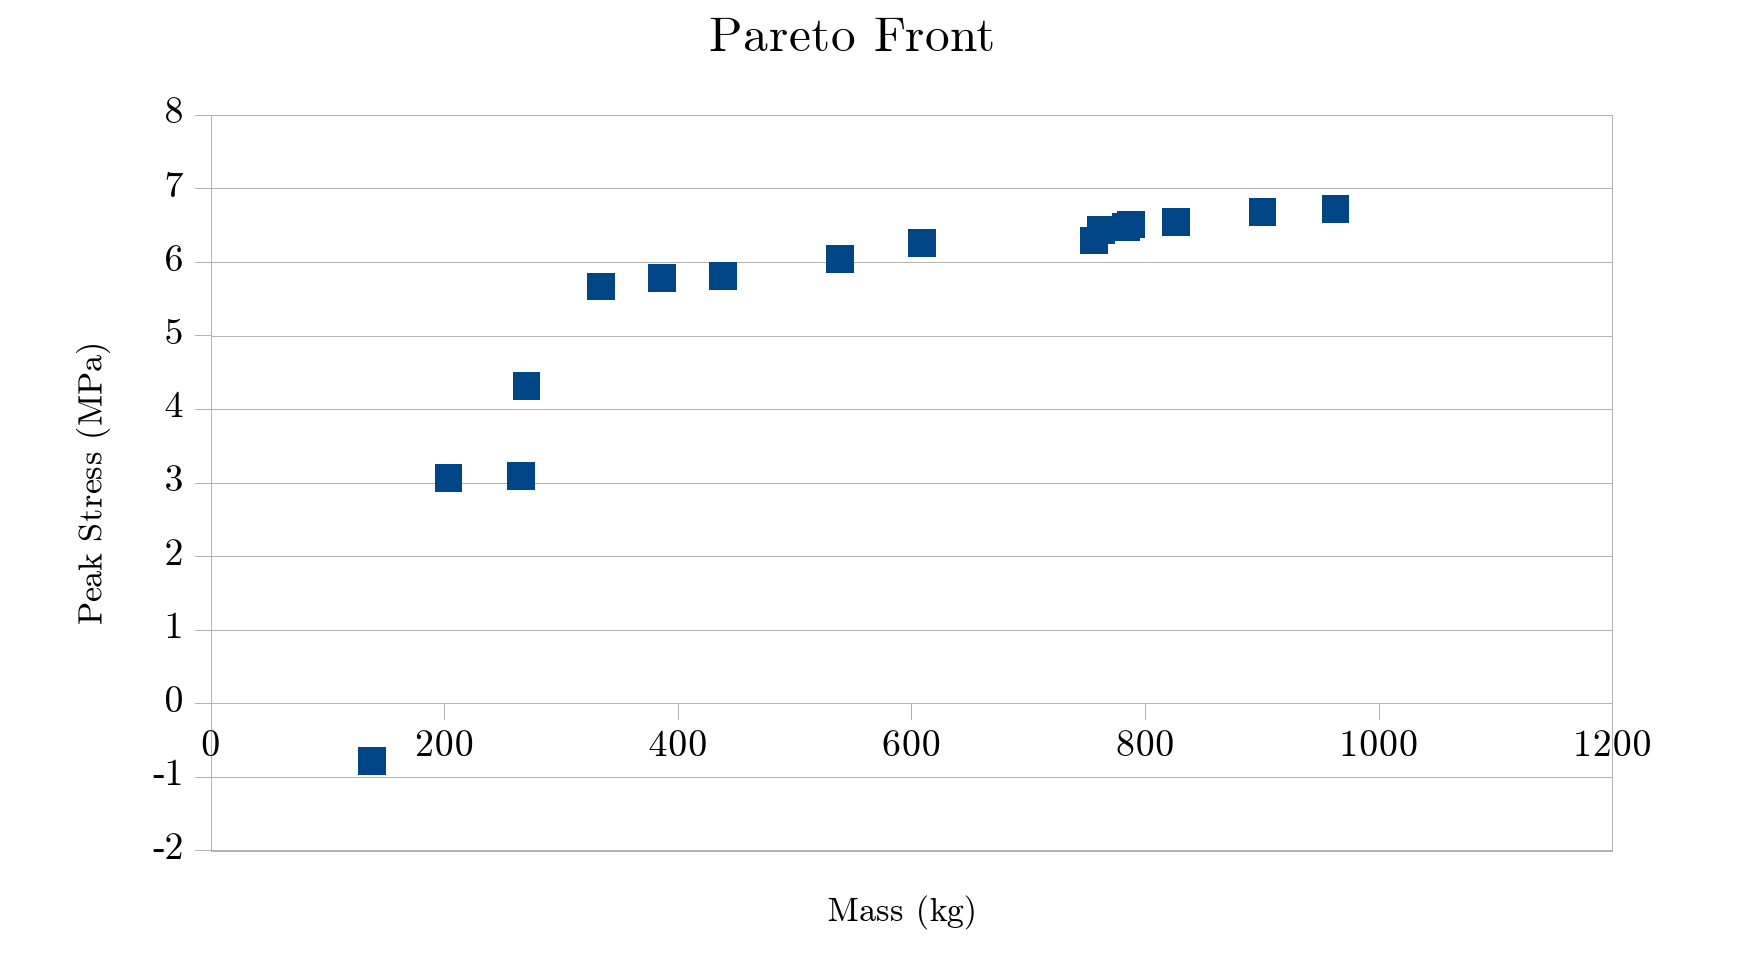
\includegraphics[width=\textwidth]{img/s3i80g200_front.png}
	\caption{Graph of the Pareto Front generated through Stochastic Loads (Short Run)}
\label{fig:pfront_sto_short}
\end{figure}

\subsection{Solution Statistics}
This solution also was tracked for several computing performance indicators to compare the performance of the algorithm with the other solutions. These statistics are listed in Table \ref{tab:stat_sto_short}. 

\begin{table}[!htbp]
  \centering
  \begin{tabular}{|l|l|}
    \hline
	  Total Generations Computed & 200\\
    Average Time Per Generation (sec) & 44.6\\
    Total Wall Clock Time (sec)	 & 8.92E+03\\
    \hline
  \end{tabular}
	\caption{Solution Statistics for Stochastic Loads (Short Run)}
  \label{tab:stat_sto_short}
\end{table}
